\title{STermWare: brief semantics description}
\author{
        Ruslan Shevchenko \\
                ruslan@shevchenko.kiev.ua\\
        Kiev, Ukraine
}
\date{\today}



\documentclass[12pt]{article}
\usepackage{listings}
\usepackage{amsmath}
\usepackage{pgf}
\usepackage{tikz}
\usetikzlibrary{arrows,automata}

% "define" Scala
\lstdefinelanguage{scala}{
  morekeywords={abstract,case,catch,class,def,%
    do,else,extends,false,final,finally,%
    for,if,implicit,import,match,mixin,%
    new,null,object,override,package,%
    private,protected,requires,return,sealed,%
    super,this,throw,trait,true,try,%
    type,val,var,while,with,yield},
  otherkeywords={=>,<-,<\%,<:,>:,\#,@},
  sensitive=true,
  morecomment=[l]{//},
  morecomment=[n]{/*}{*/},
  morestring=[b]",
  morestring=[b]',
  morestring=[b]"""
}



\begin{document}
\maketitle

\begin{abstract}
 Termware is a term rewriting system which implemented as internal and external DSL.
\end{abstract}

\section{Motivation}

  Rule-based deduction and rewriting is a well known techniques. Exists many formalizations, from
  equational logic to $\rho$-caclulus \cite{RhoCal-Wrla2002} and pure pattern calculus\cite{Jay05purepattern}   Few programming languages are build on top of rule rewriting technique.

  We need compact and clean formalizm for definition of programming language construction. Classical term
 rewriting can be used for describing program transformations 'in small', but leave dealing with context out 
 of scope of analysis. Exists different approaches for solving such issues: program analyzers based on 
 termware framework \cite{DBLP:journals/fuin/DoroshenkoS06} uses terms enriched by context parameters wich provide
 API for quering semantics properties, Statego\cite{BravenboerKVV08} use dynamic context-specific rules.

 Another approaches is hight order abstract syntax\cite{Pfenning:1988:HAS:53990.54010}: AST with binding information encoded as lambda terms, where binded names represented as binded variables.  

 Our proposed approach is an algebra of context-depended term, where operations under term with context are expressed in explicit form.

\section{Basic definitions}

   Let's build term algebra on top of some set of constants, which constists from
\begin{itemize}
 \item original constants ${c_i} \in C$ Also we
 will need to distinguish some special subset of constants: atoms ${a_i}$ and also have some special set 
of atoms.
 \item functional term $f_i \in F$  i.e. if $f \in F, c_i \in T (i \in 1..n)$, then $f(c_{1} \dots c_{n}) \in T$
 %\item variable terms $x_{i}$ which can be inside variable-bound terms.
 \item rule terms in form $\eta x_1 \dots x_n : p_{1} \to r_1 | p_2 \to r_2 | \dots ! p_{k}$
 %\item variable bounds term, i.e. so-called 'with-expressions': $with(x_1 \to t_i,\dots x_n\to t_n):t$
 %\item rule terms, i. e. so-called 'rule expressions': 
 %      $rule(p_1 \to r_1; p_2 \to r_2 ; \dots p_n \to r_n : p_{fail})$
 \item application $a b$
 \item context-terms in form of $context(a,b)$ where $a$ is $rule-term$ which can be  delayed operation
 \item set-term $\{ t_1 \dots t_2 \}$ which define set of term. Also, let's define special atom for empty
  set: $\emptyset$ and for universum $U$
\end{itemize}

 And set of usual term operations:
 \begin{itemize}
   \item subterm:  
        $$ \left.\begin{array}{l}
           subterm(f(t_1,..t_n),i)=x_i  \\
           subterm(context(S,t),i)=context(S,subterm(t,i)) \\
           subterm(\{t_1 \dots t_n \},i)=\{subterm(t_1,i), \dots subterm(t_n,i)\}  \\
           subterm(F,i)=\emptyset \\
           \end{array}\right.
        $$
   \item union: $ x | y = \{ x, y \}$
        $$ \left.\begin{array}{l}
             x | \emptyset = x  \\
             U | x = U \\
             {x | x } = x \\
	     \{ x \to a, x \to b \} = x \to \{a,b\} \\
             \{ x \to a, y \to a \} = \{ x, y\} \to a \\
             context(c,x) | context(c,y) = context(c, x|y) \\
           \end{array}\right.
        $$
       also we will identify term and one-element set.

   \item intersection: $ x \& y $
        $$ \left.\begin{array}{l}
             x \& \emptyset = \emptyset  \\
             U \& x = x \\
             {x \& x } = x \\
             x \to a \& x \to b  = x \to a \& b \\
             (a | b ) \& c = a\& c | b\&c \\
             (a \& b ) | c = a\& c | b\&c \\
           \end{array}\right.
        $$
         Also usefule will be notation $\langle x_1 \dots x_n \rangle$ wich we will call 'compatible set'.

         
   \item substitution and unification:  
        Note, that in out formalizm substitution and unification results can be represented as ordinary terms
        (set of arrows). Also note, that we can any term $t$ repesent as arrow $\emptyset \to t$, by
        (let's name on 'substituion term')
        $$ subst(x,y) = 
           \left\{\begin{array}{l l l }
             x=\emptyset &             & \emptyset \\
                         & y=\emptyset & x \\
             x           & y=a_{y} \to b_{y} & subst(b_{y},unify(x,a_{y})) \\
           \end{array}\right.
        $$

        $$ unify(x,y) = 
           \left\{\begin{array}{l l l }
             x=\emptyset &              & \emptyset \\
             x           & \emptyset    & \emptyset \\
              c_i \in C  &    c_j \in C & c_i == c_j \\
              a -> b     &              &  \\
           \end{array}\right.
        $$
        
 \end{itemize}


  Transformations:

\begin{itemize}
     \item application reduction
           $$ (\eta x_j : p_i \to r_i| \dots ! p_{fail} ) q = 
                    \left\{\begin{array}{l l}
                             \sigma r_i & \text{if $\sigma=\text{unify}(p_i,q)/x_{i}$} \\
                             p_{fail}   & otherwise \\
                           \end{array}
                    \right\} 
           $$
     \item application 
           $$
             (a->b) c = \left\{
                          \begin{array}{l l}
                             sigma b & \text{ if $\sigma=\text{unify}(a,c) $  }
                          \end{array}{l l}
                        \right\}
           $$
\end{itemize}


\subsection{ Matching Net }

  For effecient 

for example, next term

$$
 \begin{aligned}
  \eta x, y: & f(x,g(y),x)  \to {p_1}(x,y) | \\
                    & f(x,x,x)      \to {p_2}(x) | \\
                    & f(x,y,x)      \to {p_3}(x,y) | \\
                    & g(y)         \to y | \\
                    & x \to A \\
 \end{aligned}       
$$

 will be represented by matching net, shown below:

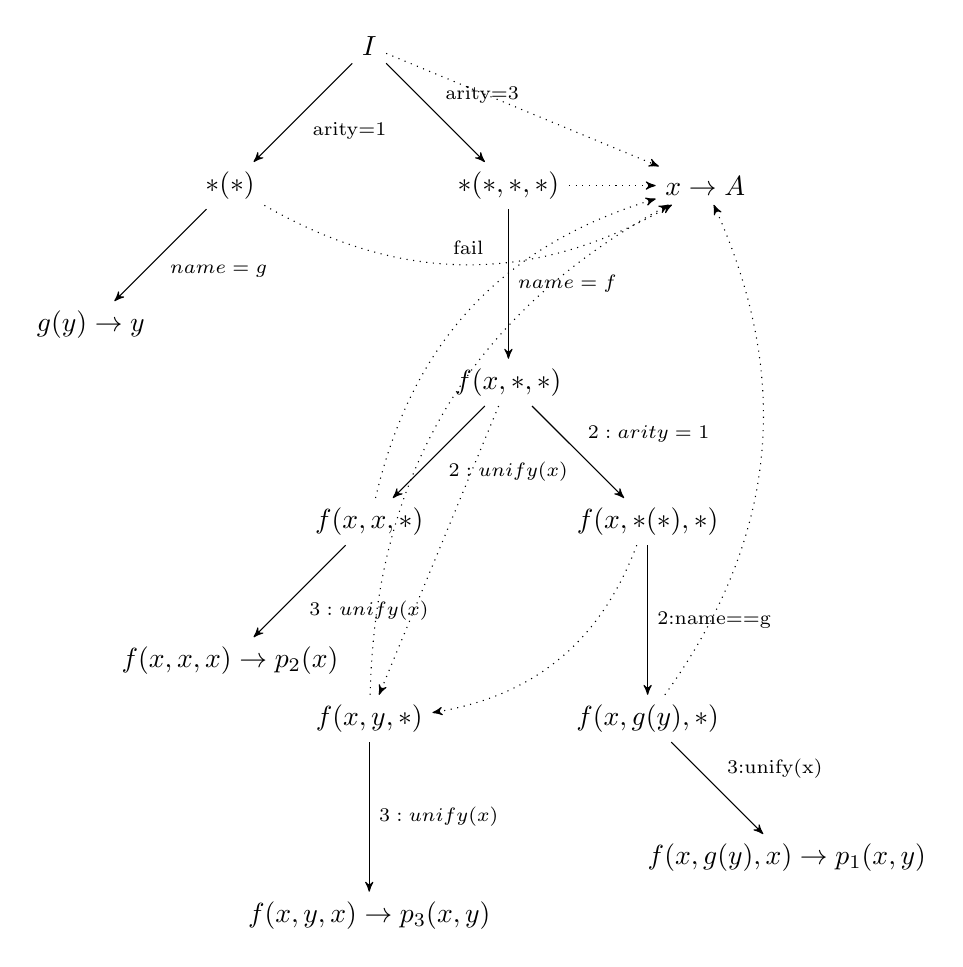
\begin{tikzpicture}[->,>=stealth',auto,node distance=2.5cm]
  
  \node(initial, state) (I)    { $I$ };
  \node(state)          (3)    [below right of=I] { $*(*,*,*)$ };
  \node(state)          (3fx)  [below of=3]   { $f(x,*,*)$ };
  \node(state)          (3fx1) [below right of =3fx ] { $f(x,*(*),*)$ };
  \node(state)          (3fx1gy) [below of =3fx1 ] { $f(x,g(y),*)$ };
  \node(state)          (3fx1gyx) [below right of=3fx1gy]  {$f(x,g(y),x) \to p_1(x,y)$ };
  \node(state)          (3fxx) [below left of=3fx]  { $f(x,x,*)$ };
  \node(state)          (3fxxx) [below left of=3fxx]  { $f(x,x,x) \to p_2(x)$ };
  \node(state)          (3fxy) [below  of=3fxx]  { $f(x,y,*)$ };
  \node(state)          (F)     [right of=3]  { $x \to A$ };
  \node(state)          (3fxyx) [ below  of=3fxy ] { $f(x,y,x)\to p_3(x,y)$ };
  

  \node(state)          (1) [below left of=I]     { $*(*)$ };
  \node(state)          (1gy) [below left of=1]      { $g(y) \to y$ };


  \path[font=\scriptsize]
          (I)    edge node { arity=3 }  (3)
               edge node { arity=1 }   (1)
                edge [dotted] node  { } (F)
         (3)   edge node { $name=f$ }  (3fx) 
                 edge [dotted] node { }   (F)
       (3fx)  edge node { $2:arity=1$ }  (3fx1)
                 edge node { $2:unify(x)$ }  (3fxx)
                 edge [dotted] node { } (3fxy)
       (3fxx) edge node { $3:unify(x)$}  (3fxxx) 
                 edge [bend left,dotted] node  { } (F)         
       (3fx1) edge node {2:name==g } (3fx1gy)
                  edge [bend left, dotted] node { } (3fxy)
       (3fxy)  edge node {$3:unify(x)$}  (3fxyx)
                  edge [bend left,dotted] node { } (F)
       (3fx1gy)  edge node {3:unify(x)}  (3fx1gyx)
                  edge [bend right,dotted] node { } (F)
        (1)   edge node {$name=g$}  (1gy)         
                edge [bend right,dotted] node {fail}  (F) 
        
           ;

\end{tikzpicture}

 Here, each node match imply one lookup (via arity or via name) and then match the rest of target term with the received node; on success we will reach termination node; on failure -- exclude looked patch from possible termination and retry unification until termination patch will be found or all possible forward patched exhausted.  If not forward unification is possible in the given node - navigate to next candidate via fallback edge (which are shown as dotted on the scheme).


\bibliographystyle{abbrv}
\bibliography{stermware}

\end{document}
